\chapter{Introduction} \label{chap:intro}
The goal of this thesis is the implementation of a parallel implementation of a pointer analysis. As well as researching to what extent such an implementation presents advantages or disadvantages over other analyses that are not strictly parallel in nature.

\section{Structure of this Thesis}
This thesis is divided into three chapters.
The first chapter \autoref{chap:intro} lays the groundwork for the implementation and goes into detail what ideas were persued in order to develop the implementation. All related current work and it's influences on this work is discussed here, as well as the motivation for the implementation itself. Furthermore the fundamentals of pointer analysis are explained here with code samples and an end to end analysis workflow that aims to illustrate the connection between actual code and its representation in a pointer analysis.

In the second chapter \autoref{chap:main} the software, namely PTAGPU, that was developed as part of this thesis, is described in detail. Design decisions, integrations with other software libraries and correctness are elaborated here.
The experimental benchmark results and how they wre generated are also presented here.

The last chapter \autoref{chap:conclusion} covers possible future work that could further improve the implementation and explore more ideas concerning parallel pointer analyses.
This chapter also discusses the experimental results from \autoref{chap:main}.

\section{Motivation}
general alias analysis is undecidable
This thesis aims to explore the possibilities of parallelizing the Andersen style inclusion based whole program pointer analysis. The goal is to improve static pointer analysis performance by using massively parallel GPUs.
With the general trend of more complex software systems in software development, developers also require static analysis tools that are able to perform scalable analyses on entire codebases.
Unfortunately general pointer analysis is undecidable problem, which is a problem that prevents maximally precise pointer analysis from being a possibility.
For this reason a balance must be found between performance and precision when analyzing code.
Historically most pointer analysis solutions have been implemented as single threaded applications. By using GPGPUs the proposed library from this thesis aims to improve performance when analyzing entire programs by distributing the work accross the many streaming processors modern GPGPUs possess. The proposed performance improvement also does not decrease the analysis precision.
\subsection{Static Analysis in Software Development}
finding bugs is becoming harder

inter procedural analysis scalability; create a single machine implementation that used parallel hardware and integrates into SVF

In general a pointer analysis tries to find the values of pointers in a program at runtime, without having to execute the program.
So naturally this problem is undecidable \cite{landi1992undecidability} following a reduction from the halting problem.
As a result, performing a pointer analysis becomes a delicate balancing act between precision and peformance.
Commonly analyses produce over-approximation of the targets each pointer can point towards at runtime while other parts of an analyses might omit or under-approximate certaint parts for the sake of performance and scalability.
As a result, these analyses are strictly speaking unsound or soundy as put forward by \cite{livshits2015defense}:

\begin{quote}
    We introduce the term soundy for
    such analyses. The concept of soundiness
    attempts to capture the balance,
    prevalent in practice, of over-approximated
    handling of most language features, yet deliberately
    under-approximated handling of a feature subset well
    recognized by experts. Soundiness is in
    fact what is meant in many papers that
    claim to describe a sound analysis. A
    soundy analysis aims to be as sound as
    possible without excessively compromising
    precision and/or scalability.
\end{quote}

Pointer analyses build the foundation for a variety of other static analyses, since call-graph generation is directly dependent on pointer analysis in order to resolve indirect or dynamic calls statically.

One common pointer analysis is the inclusion-based Andersen's analysis \cite{andersen1994program}. The details of this type of analysis will be discussed later on, as it is the underlying basis for the proposed algorithm in \autoref{chap:main}. The Andersen algorithm sacrifices precision in favor of performance and achives an upper bound of $O(n^3)$ where n represents the number of pointer variables relevant to the analysis. This is known as the cubic bottleneck of general Andersen analysis \cite{mathiasen2021fine}.
This showcases the tradeoff that all non-theoretical pointer analyses have to make in oder to be applicable to real programs and avoid undecidability. Furthermore Andersen's analysis is a P-complete problem and is therefore not trivially parallelizable.

As a general abstraction, pointer analyses can be seen as complex graph problems where programs are interpreted as graphs with nodes representing variables and edges representing relations between nodes, such as memory allocations and assignments bewteen variables.
This allows us to make use of a large body of previous research concerning graph problems and transform the general analysis into a better defined mathematical problem.

Another analysis closely related to pointer analysis is alias analysis, where two pointers are said to alias if their points-to sets have an intersection. An alias analysis produces a set of relations over all nodes in the analysis graph where nodes can either \textbf{NotAlias}, \textbf{MayAlias} or \textbf{MustAlias}.
For two given nodes, $a$, $b$ and their points-to sets $pts(a)$ and $pts(b)$ the following constraints describe the relations.
$$a\ \textbf{NotAlias}\ b \iff \forall ptd \in pts(a) \colon ptd \notin pts(b)$$
$$a\ \textbf{MayAlias}\ b \iff \exists ptd \in pts(a) \colon ptd \in pts(b)$$
$$a\ \textbf{MustAlias}\ b \iff \forall ptd \in pts(a) \colon ptd \in pts(b)$$
Both pointer analysis, alias analysis, as well as points-to analysis are all terms commonly used interchangeably in literature \cite{hind2001pointer}. From now on pointer analysis will be used in this thesis to refer to this type of static analysis from which an alias relation can be derived based on the pointer information.

A motivating example for pointer analyses is the detection on memory leaks in programs.
This occurs when a memory location is allocated on the heap, for example with a call to malloc in glibc, and is not freed at a later stage in the program.
It is in the interest of the developer to find such faults as to not exhaust the computers memory during execution by repeatedly allocating memory in the heap without freeing previous allocations.
Finding such logical errors can be accomplished via a related static analysis called data-flow analysis, where each possible value at different stages of the program is calculated. Here pointer information is vital, as pointers can represent lateral movement of data trough the control flow of a program, independent of direct assignments and read operations. Ultimately almost all static analyses require some kind of information about pointers to fully determine the state of a program.
Aside from error detection such as memory leaks, optimizations are another aspect of compiler systems, where pointer information is important to achieve better results, see \autoref{lst:dataflow}.
More often than not the pointer information alone does not provide an immediate value to the compiler or analysis tool, instead other procedures build on top of this information to derive valuable information about a program.

\begin{listing}
    \begin{minted}{c}
    #include <stdlib.h>
    void *iter;
    iter = value;

    /* depending on the data at value's memory location 
    the loop might not be necessary */
    
    while(*iter)
    {
        complex_computation(iter);
    }
    \end{minted}
    \caption{Optimizations in a c program}
    \label{lst:dataflow}
\end{listing}

\subsection{Notions of Sensitivity in Pointer Analysis}
As previously established, a complete pointer analysis is undecidable.
For this reason there are various notions of sensitivity when talking about pointer analysis.
These notions represent a compromise between precision, scalability and complexity of the analysis.
Following, some of the more common sensitivity notions will be illustrated to differentiate the more complex analyses from the less complex analyses and explain the impact of these sensitivities on actual performance when analyzing a program.

\subsubsection{Field-sensitivity}

\begin{listing}
    \begin{minted}{c}
    int a;
    char b;
    struct Person {
        char *name;
        int *age;
    } p1, p2;
    p1.age = &a;
    p1.name = &b;
        \end{minted}
    \caption{Field-sensitivity by example}
    \label{lst:field}
\end{listing}

Field-sensitivity describes how the pointer analysis algorithm handles structures in the program.
Most programming languages that expose memory management to a developer, such as c, c++ and Rust, offer some form of structures to represent an object that internally holds multiple values where these values might be pointers, that reference memory locations.
If an analysis is field-sensitive, each field of each struct is represented in the analysis as an independent node that can point to unique memory locations, as long as the field can be statically determined during the analysis, see \autoref{lst:field}.
If the field of a struct can not be statically determined, for example because of an arithmetic operation that produces multiple possible results for the offset during runtime, it is common for field-sensitive pointer analyses to fallback to a field-insensitive mode for the specific struct, wherein all fields of the struct are merged into a single abstract object.
For the given example, \verb|p1.age| and \verb|p1.name| can point to different memory locations.
Alternatively a field-insensitive analysis does not differentiate between any fields of a given struct at any point of the analysis.
Therefore only two nodes are created to represent the struct, $p1.*$ and $p2.*$.
Another common alternative is field-base-sensitivity, where instead of omitting the individual fields of each struct, the fields of every struct are merged into a single instance of that struct.
As a result the Person structs, p1 and p2, would be represented as a single object with fields name and age, such that \verb|p1.age == p2.age| are represented by the same node in the analysis.

\subsubsection{Array-sensitivity}
Array-sensitivity is conceptually similar to field-sensitivity but often has different effects on the runtime of the analysis.
For a given array $int arr[100]$ an array-sensitivie analysis would model each entry of the array, \newline e.g. arr[0], arr[1], \dots, with a unique node, whereas an insensitive analysis would model the array as a single node.
Generally speaking arrays are often homogeneous data structures that can hold a vast amount of data, compared to structs which are often more compact as they model attributes instead of raw data.
Therefore array-sensitivity if often omitted from whole program analyses, while field-sensitivity is common among pointer analyses.

\subsubsection{Scope of the analysis}
When designing a pointer analysis one has to make a decision about how to handle external code that the program depends on.
Often times a programs transitive dependencies can dwarf the original code by several magnitudes in size \cite{toman2017taming}.
Even a basic Hello World program in Java transitively depends on 3000 classes \cite{kulkarni2016accelerating} from the Java standard library.
For this reason most analyses either ignore external library code during analysis, or stub the most relevant library calls during analysis, such as \verb|malloc| or \verb|free|.
This tradeoff is well worth it, as most interesting properties in pointer analysis do not originate in extenal libraries, but the actual program code that is written by the developer.
This does however not solve the problem of standard library code mutating the program state either via callbacks or mutation of values behind pointer arguments. Here, simply ignoring the external code during analysis would greatly decrease the accuracy of the analysis.
For this reason, a lot of research is being done to develop methods that alleviate some of the problems that arise from analyzing external dependencies of a given program. Caching incremental results during analysis seems to be one of the most promising methods thus far \cite{mcpeak2013scalable}, where instead of solving the pointer analysis problem from the top-down, the analysis begins at the bottom and builds summaries for functions incrementally until a result over the entire program is achieved. Hybrid approaches combining top-down and bottom-up analysis represent state of the art analysis methods in use by production static analysis tools, such as Coverity \cite{mcpeak2013scalable}.

\subsubsection{Interprocedural analysis}
Another aspect that greatly influences the precision of analyses is whether they are interprocedural or intraprocedural.
An intraprocedural analysis only analyzes each function in an isolated context and disregards any influences on other functions or global state.
Interestingly most compilers rely mostly on intraprocedural analysis for bug detection as it can be performed in parallel for each function independently and is in general much faster than interprocedural analysis.
The following example \ref{lst:intraprocedural} illustrates the shortcomings of only performing intraprocedural analysis. Essentially parameter passing especially of pointers is not taken into account properly for the calculation of points-to sets.
An interprocedural analysis overcomes these limitations by connecting parameters of functions and the arguments at the respective callsites as well as the resulting return values in the graph structure that is used to solve the pointer analysis.
Fundamentally an interprocedural analysis is related to another notion of sensitivity, context sensitivity, since every context sensitive analysis has to be interprocedural in order to capture the context of each function call \cite{lin2015alias}.

\begin{listing}
    \begin{minted}{c}
        int *manupulatePointer(int *ptr);
        int main() {
            int *a, *b;
            b = manupulatePointer(a);
            /* intraprocedural analysis is unable 
            to determine the state of a or b */
        }
    \end{minted}
    \caption{Limitations of intraprocedural analysis}
    \label{lst:intraprocedural}
\end{listing}

\subsubsection{Flow-sensitivity}
When one performs a flow-sensitive pointer analysis, this means that the analysis takes into account the control flow of the program when calculating point-to information.
As can be seen in \ref{lst:flowsens}, a flow-sensitive analysis is in general more precise than a flow-insensitive analysis. Meanwhile running a flow-sensitive analyis is also exponentially more expensive to compute as every step in a programs control flow carries its own state concerning points-to relations - especially when the control flow is complicated by complex conditional statements or recursive execution.
Although this problem can be slightly alleviated, by only condering program statements that manipulate pointers.
Using a flow-sensitive pointer analysis also generates must-alias relations, compared to the comparatively imprecise may-alias relations from a flow-insensitive pointer analysis.
Generating definitive information that two variables will unconditionally alias during runtime is very valuable when considering refactoring optimizations by a compiler.
While a sound may-alias analysis requires that no possible alias relations are missed, a sound must-alias analysis requires analogously that no spurious alias relations are reported. Both are respectively over- and under-approximations of the true points-to results.

\begin{listing}
    \begin{minted}{c}
        int *manupulatePointer(int *ptr);
        int main() {
            int a, b, *x; // x -> {}
            if (something())
                x = &a; // x -> {a}
            else
                x = &b; // x -> {a,b} ?
            manupulatePointer(x);
            /* a flow insensitive analysis computes 
            a points-to set {a,b} for x while in actuality 
            x = &b and x = &a are mutually exclusive statements
            during execution */
        }
    \end{minted}
    \caption{Flow-sensitivity by example}
    \label{lst:flowsens}
\end{listing}

\subsubsection{Context-sensitivity}
As previouly eluded to, context-sensitivity is directly related to interprocedural analyses, since it governs how call sites and called functions are interpreted during the analysis.
More specifically a centext-sensitive analysis tries to qualify variables both on the heap and stack with contextual information such that different contexts can be established, where for example points-to information for a variable differs, thus improving the precision of the analysis.
To achieve this context-sensitivity can be modeled by using call-sites and objects to differentiate qualify the context for variables \cite{smaragdakis2015pointer}. Depending on the programming language at hand, these methods can yield different precision. It has been established that object oriented languages like Java greatly benefit from object-sensitivity over call-site-sensitivity, while more procedural languages like C benefit from call-site-sensitivity.
While a context-sensitive analysis would in theory provide more precision and therefore decrease the average size of points-to sets, in practice most context-sensitive pointer analyses, when applied to sizeable codebases, quickly grow out of control as the analysis explodes in terms of running time and space requirements \cite{smaragdakis2014introspective}. In contrast, context-insensitive analyses anecdotally scale better than context-sensitive analyses.

\begin{listing}
    \begin{minted}{c}
        int *manupulatePointer(int *ptr);
        int main() {
            int a, b, *x;
            x = &a;
            manupulatePointer(x);
            x = &b;
            manupulatePointer(x);
            /* a context-sensitive analysis evaluates both
            calls to manupulatePointer as unique function calls
            since the context differs between both calls */
        }
    \end{minted}
    \caption{Context-sensitivity by example}
    \label{lst:contextsens}
\end{listing}

\subsection{Andersen's Analysis}
Andersen's analysis is an inclusion based interprocedural pointer analysis algorithm first proposed by \cite{andersen1994program} in 1994. It is a field-sensitive, context-insensitive and flow-insensitive analysis. 
The algorithm was one of the first constraint based algorithms introduced for pointer analysis. Since it is lacking constext- and flow-sensitivity, it is often used as a base algorithm which produced broad over estimations of the points-to data and is later refined by more precise algorithms which improve the quality of the data and remove false positives from the points-to information generated by Andersen's algorithm.
The underlying idea is that the Algorithm operates on a given program by converting statements from the program into mathematical constraints contained in a constraint graph.
These constraints can be classified into a few types which can be seen in \autoref{tab:ander}.
It is worth noting that in literatur the field-sensitivity aspect is often omitted from the definition of the Andersen analysis although it was included in the original specification.
As mentioned in \autoref{chap:intro} the complexity of Andersen's analysis grows exponentially with regards to the number of pointer variables in a program. The reason for this exponential growth, among other aspects, is the field-sensitivity. Depending on the structure of the code under analysis, field-sensitivity might play the most influential part in the analysis' complexity. This will be further expanded upon in \autoref{chap:main}. Ultimaltely this is the reason for specifically including field-sensitivity when discussing Andersen's analysis in this thesis.
During execution an Andersen style pointer analysis repeatedly applies the constraints until a point is reached where no more changes are applied to the constraint graph at which point the execution concludes and the points-to sets for each variable are returned.
\begin{table}
    \begin{center}
        \caption{Constraints of an inclusion-based pointer analysis.}
        \label{tab:ander}
        \begin{tabular}{l|l|c|l}
            \hline                                                                                                                         \\
            \textbf{Statement} & \textbf{Name} & \textbf{Description}                        & \textbf{Constraint}                         \\
            \hline                                                                                                                         \\
            $x = \&a$          & alloca        & The address of a is assigned to variable x. & $\{a\} \subseteq pts(x)$                    \\
            $x = y$            & copy          & Variable y is assigned to x.                & $pts(y) \subseteq pts(x)$                   \\
            $x = *y$           & load          & Load value of y and assign to x.            & $\forall p \in pts(y) \colon p \subseteq pts(x)$ \\
            $*x = y$           & store         & Store y into value of x.                    & $\forall p \in pts(x) \colon y \subseteq pts(p)$ \\
            $x = y.f$          & field         & Field f of variable y is assigned to x      & $pts(y.f) \subseteq pts(x)$                 \\
        \end{tabular}
    \end{center}
\end{table}

\subsection{Steensgard's Analysis}
Steensgard's analysis was introduced in 1996 by \cite{steensgaard1996points}. It was inspired by Andersen's analysis and as such is also an interprocedural pointer analysis.
The key proposition of Steensgard's work was to improve the runtime of Andersen's algorithm by using equalities instead of subsets for the constraints that are used as inputs for the algorithm, an overview for the constraints can be seen in \autoref{tab:steens} - the rules are nearly identical to the constraints for the Andersen algorithm.
The change from subsets to equalities leads to an almost linear algorithm by utilizing union/find data structures for efficient computation of a fixpoint solution for a given set of pointers.
The tradeoff for this faster algorithm is precision, since Steensgard's algorithm quickly looses precicion compared to Andersen's algorithm by loosing the small differences between points-to sets of individual varialbes by equating them. An example for this precision loss can be seen in \autoref{lst:steensvander}.

\begin{listing}
    \begin{minted}{c}
        int main() {
            int a, b, *x, *y;
            x = &a; // pts(x) = {a}
            y = &b; // pts(y) = {b}
            y = x; // pts(y) = pts(x) = {a,b}
            /* by equating the points-to sets of x and y
            the fact that x never points to b is lost
            this leads to an obvious loss of precision */
        }
    \end{minted}
    \caption{Steensgard easily looses precision.}
    \label{lst:steensvander}
\end{listing}

\begin{table}
    \begin{center}
        \caption{Constraints of an equality-based pointer analysis.}
        \label{tab:steens}
        \begin{tabular}{l|l|c|l}
            \hline                                                                                                                 \\
            \textbf{Statement} & \textbf{Name} & \textbf{Description}                        & \textbf{Constraint}                 \\
            \hline                                                                                                                 \\
            $x = \&a$          & alloca        & The address of a is assigned to variable x. & $pts(x) = \{a\} \cup pts(x)$        \\
            $x = y$            & copy          & Variable y is assigned to x.                & $pts(y) = pts(x)$                   \\
            $x = *y$           & load          & Load value of y and assign to x.            & $\forall p \in pts(y) \colon p = pts(x)$ \\
            $*x = y$           & store         & Store y into value of x.                    & $\forall p \in pts(x) \colon y = pts(p)$ \\
            $x = y.f$          & field         & Field f of variable y is assigned to x      & $pts(y.f) = pts(x)$                 \\
        \end{tabular}
    \end{center}
\end{table}

\subsection{Wave Propagation}
Since its first introduction in 1994, there have naturally been many incremental improvements to Andersen style pointer analysis.
Most current implementations are derived from \cite{waveprop}, specifically the Wave Propagation Method, which is a highly optimized version of Andersen's algorithm.
In Wave Propagation the procedure is separated into an insertion phase and a propagation phase. Furthermore the constraint graph is topologically sorted and acyclic, which enables the algorithm to pass forward the computed points-to information in topological order, preventing redundant work since only set differences need to be propagated to the next nodes. The algorithm is intended to be more memory intensive in order to achieve better performance on large codebases \cite{waveprop}.
The general algorithm for wave propagation is listed in \autoref{alg:waveprop}.

\begin{algorithm}
    \caption{General Wave Propagation Algorithm \\ \textbf{Input:} Constraint Graph $G=(V,E)$ \\ \textbf{Output:} Modified Constraint Graph $G=(V,E)$ and points-to information for each node.}\label{alg:waveprop}
    \begin{algorithmic}
        \State Detect strongly connected components and find topological sorting for $G$. \\ Build topological node stack $T$.
        \Repeat
        \State changed = False
        \State worklist = $\emptyset$
        \While{$T \neq \emptyset $}
        \State node $\leftarrow$ pop from T
        \For{edge (node,target) $\in out_{copy/gep}(node)$}
        \State pts(target) $\leftarrow$ union pts(node) pts(target)
        \If{pts(target) changed}
        \State changed = False
        \State add target to worklist
        \EndIf
        \EndFor
        \EndWhile
        \While{worklist $\neq \emptyset $}
        \State node $\leftarrow$ pop from worklist
        \For{edge (node,target) $\in out_{load}(node)$}
        \For{ptsDst $\in pts(node)$}
        \State add copy edge (ptsDst, target) to $G$.
        \If{edge added to $G$}
        \State changed = True
        \EndIf
        \EndFor
        \EndFor
        \For{edge (src,node) $\in in_{store}(node)$}
        \For{ptsDst $\in pts(node)$}
        \State add copy edge (src, ptsDst) to $G$.
        \If{edge added to $G$}
        \State changed = True
        \EndIf
        \EndFor
        \EndFor
        \EndWhile
        \If{Edge added to $G$}
        \State changed = True
        \EndIf
        \Until{changed = False}
    \end{algorithmic}
\end{algorithm}

\subsection{LLVM - Generating Data for Analysis}
By now the fundamentals of pointer analysis have been introduced, which unilaterally can be modeled as a graph problem.
The missing part of the Introduction is where the underlying data for such a pointer analysis algorithm comes from or how it is derived from a given program that has to be analyzed.
Initially pointer analyses were solely implemented in compilers to detect errors and find possible optimizations during compilation. As compilers already employ an internal representation for the programs to be compiled, the data generation was not problematic.
As the scope of pointer analyses expands from intraprocedural analysis part of a compiler towards standalone interprocedural whole program analyses it is clear, that a new representation for programs is needed, on which analyses can run - independent of compilations.

During initial review of literature for pointer analysis multiple methods for data generation were surveyed. Notably parsing was among the most common data extraction methods for programs. Another method was to extract an intermediate representation, called LLVM-IR, of the code during compilation of a program by means of using the low level virtual machine, LLVM. Using LLVM has some distinct advantages compared to parsing the source files of a program directly.
For one, LLVM provides multiple compiler front-ends for various compiled programming languages, including C/C++ and Objective-C through the Clang compiler, which allows one to compile multiple languages without having to adapt the parser, as can be seen in \autoref{fig:llvm}.
Especially when working with older non-strictly standardized versions of the C language, utilizing all available tricks of an established compiler proves to be more resourceful compared to reinventing the wheel with new parsing tools.
Secondly one can easily verify the correctness of the extracted data for a program by simply executing the compiled intermediate representation since no matter the programming language, as part of the llvm toolchain the program always gets compiled into the intermediate representation before being assembled and linked. The LLVM project provides specific tools for executing programs in LLVM-IR format using a just-in-time compiler \footnote{https://releases.llvm.org/9.0.1/docs/CommandGuide/lli.html}. Beyond the binary intermediate representation, also called bitcode, there exists a human-readable format. Both binary and text versions can be converted between with the llvm tools \verb|llvm-as| and \verb|llvm-dis|, see \autoref{lst:llvmir} for a basic hello world program in human-readable LLVM-IR.

\begin{figure}
    \centering
    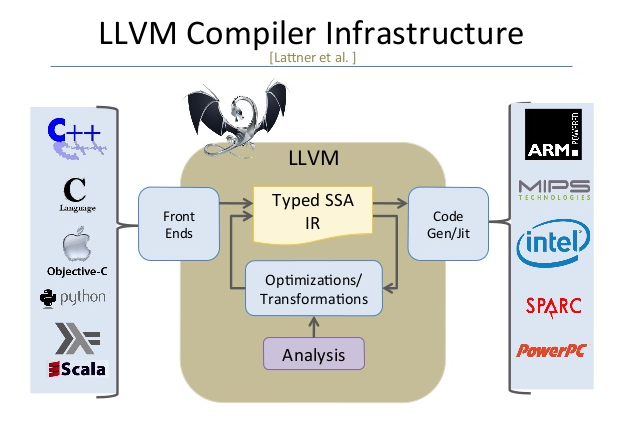
\includegraphics[width=.8\textwidth]{img/llvm.png}
    \caption{Illustration of the LLVM toolchain from Lattner et al.}
    \label{fig:llvm}
\end{figure}

\begin{listing}
    \begin{minted}{c}
#include <stdio.h>
int main()
{
    int i;
    i = 10;
    printf("Hello World! N = %d\n", i);
    return 0;
}
// gets compiled into...
    \end{minted}
    \begin{minted}{llvm}
@.str = private unnamed_addr constant 
    [21 x i8] c"Hello World! N = %d\0A\00", align 1
; Function Attrs: noinline nounwind optnone uwtable
define dso_local i32 @main() #0 {
  %1 = alloca i32, align 4
  %2 = alloca i32, align 4
  store i32 0, i32* %1, align 4
  store i32 10, i32* %2, align 4
  %3 = load i32, i32* %2, align 4
  %4 = call i32 (i8*, ...) @printf(i8* getelementptr inbounds 
        ([21 x i8], [21 x i8]* @.str, i64 0, i64 0), i32 %3)
  ret i32 0
}
declare dso_local i32 @printf(i8*, ...) #1
    \end{minted}
    \caption{A basic hello world program in human-readable LLVM-IR.}
    \label{lst:llvmir}
\end{listing}

\subsubsection{LLVM Instructions}
With the generated LLVM-IR we can now build a graph, by interpreting the individual LLVM instructions as constraints for a chosen pointer analysis.
The LLVM-IR uses static single assignment (SSA) form for variables meaning that each variable can only be assigned a single time in a specific control flow in the intermediate representation.
The use of SSA form is not directly relevant to Andersen style analyses but simplifies working with variables conceptually, since no variable can be reassigned at any point of the program.
At this point it is also important to differentiate between address-taken variables and top-level variables.
Top-level variables' values reside in registers and are conceptually ephemeral while address-taken variables are abstract memory objects which logically reside in memory. The specifics of memory locations and cpu registers are of cause hardware specific and depend on the target architecture that the llvm backend assembles the intermediate representation into.
The connection between address-taken and top-level variables in the LLVM-IR is established by the \verb|alloca| instruction which maps a top-level variable to a memory location represented by an address-taken variable.
Following is an interpretation of the LLVM instructions for Andersen's pointer analysis.

\paragraph{Load Instruction}
The LLVM \verb|alloca| instruction is used to allocate memory on the stack.
\begin{minted}{llvm}
    ; allocate a pointer to a 32 bit integer on the stack 
    ; and save a reference at ptr
    %ptr = alloca i32*, align 8
\end{minted}
The analog of the \verb|alloca| instruction in a pointer analysis is the address-of operation $x = \&a$, since the top-level variable $ptr$ points to the abstract memory location holding the actual value.
This might come as a surprise, since the implementation of $x = \&a$ in C does not result in an \verb|alloca| instruction. This often leads to confusion when interpreting points-to results that are built using the LLVM-IR.

\paragraph{Load Instruction}
The LLVM \verb|load| instruction loads the value on a top-level variable into a new variable. Compared to the C programming language this is comparable to dereferencing a pointer variable.
\begin{minted}{llvm}
    %ptr = alloca i32*, align 8
    ; load the pointer to the 32 bit integer from ptr into %var
    %var = load i32*, i32** %ptr, align 8
\end{minted}
When interpreting LLVM load instructions for a pointer analysis, we can treat it as the complex load constraint that is already defined for Andersen's analysis in \autoref{tab:ander}.
Again just like the alloca instruction we can not draw a direct comparison between the definition of the constraint $x = *y$ and the equivalent statement in the C language, since we are working with the LLVM-IR in SSA form.
The C equivalant would be the dereferencing of $*y$ alone. The assignment to x would require another store instruction.

\paragraph{Store Instruction}
The LLVM \verb|store| instruction stores a value into a variable. The variable might be a top-level or an abstract memory object represented by an address-taken variable.
\begin{minted}{llvm}
    %ptr = alloca i32*, align 8
    %var = load i32*, i32** %ptr, align 8
    ; store the literal value 10 into %var
    store i32 10, i32* %var, align 4
\end{minted}
The interpretation of the LLVM store instruction is similar to the load instruction. It can be interpreted as the complex store constraint defined as part of Andersen's analysis.

\paragraph{Getelementptr Instruction}
The LLVM \verb|getelementptr| or \verb|gep| instruction is used to get subelements from an aggregate data structure such as arrays or structs. When the gep instruction is invoked, it requires an index in order to perform the address calculation for the subelement. Getelementptr does not access memory, it only finds the correct address.
\begin{minted}{c}
    int arr[10];
    arr[5] = 10;
\end{minted}
\begin{minted}{llvm}
    ; create an integer array
    %arr = alloca [10 x i32], align 16
    ; get the address for the 5th element
    %idx = getelementptr inbounds [10 x i32], [10 x i32]* %arr, 
        i64 0, i64 5
    store i32 10, i32* %idx, align 4
\end{minted}
Since we intend to run a static analysis, we need to consider the properties of the index value passed into the getelementptr instruction.
Either the index is a constant value, and we can forward the gep instruction together with the constant index into the static analysis,
or the index is a variable that is subject to change during execution, and we need to assume that every possible value can be realized during execution, i.e. every offset for an aggregate data structure might be referenced by such a gep instruction and this information must be passed to the static analysis.
This behaviour is handled by differentiating between two types of gep constraints in the pointer analysis, normal- and variant-gep constraints. The former specifying a singular offset and the latter every possible offset for a given aggregate data type, since the value can not be statically determined.

\paragraph{Copy Instruction and equivalant Instructions}
Other than the complex store, load and the address-of constraints, the Andersen inclusion-based pointer analysis operates also on simple constraints, see line 2 in \autoref{tab:ander}. In terms of LLVM-IR instructions we are only interested in those instructions that manipulate pointers. In the LLVM-IR specification lots of instructions can result in values being moved, including pointers. Therefore we group those instructions that can move values between symbols under the simple inclusion-based constraint.
The following instructions are interpreted as simple constraints:
\begin{itemize}
    \item \verb|Phi| instructions are part of the LLVM-IR to correctly resolve control flow. Depending on the conditional branch a new SSA variable is introduced that holds the resulting value from the branch.
          Since we are implementing a flow-insensitive pointer analysis we do not differentiate between constrol flows and simply interpret each phi instruction as a simple constraint connecting the conditional values to the resulting phi variable.
    \item \verb|Select| instructions serve a similar purpose as phi instructions. Here a value is selected conditionally without creating branches. As such we interpret the select instruction as a simple constraint.
    \item \verb|Call| instructions represent a function call. If the function call contains arguments the caller arguments and callee parameters need to be interpreted as a simple constraint. Beyond this, nothing is done to analyze the context of the function call, since we are performing a context-insensitive pointer analysis.
    \item Like the call instructions, \verb|Ret| instructions are simply interpreted as simple constraints so the returned function value is included in the pointer analysis.
    \item \verb|ThreadFork| \verb|ThreadJoin| are not LLVM-IR instruction. But just like the call and ret instructions, these must be interpreted as function calls with simple constraints in the context of pointer analysis.
    \item Lastly there are various instructions that are straightforward to interpret as simple constraints, including \verb|bitcast|, \verb|ptrtoint| and \verb|freeze| instructions. Furthermore variable argument values and external library call parameters need to be handled like regular call instructions.
\end{itemize}

Now with alloca, load and store instructions introduced, we can analyze a basic example during pointer analysis.
We are going to observe a simple c program:
\begin{minted}{c}
    int *p, x, *q;
    p = &x;
    q = p;
\end{minted}
Which will compile into the following LLVM-IR:
\begin{minted}{llvm}
    %1 = alloca i32*, align 8
    %2 = alloca i32, align 4
    %3 = alloca i32*, align 8
    store i32* %2, i32** %1, align 8
    %4 = load i32*, i32** %1, align 8
    store i32* %4, i32** %3, align 8
\end{minted}
An example for applying the constraint rules according to the Andersen algorithm in \autoref{tab:ander} can be observed in \autoref{tab:applyander}.
The edge labels of the constraint graph are \verb|p|, \verb|s|, \verb|l|, \verb|c| corresponding to points-to (inverse alloca), store, load and copy constraints.
Furthermore the copy edges are immediately converted into point-to edges in order to simplify the constraint graph.

\begin{table}[H]
    \caption{Applying Andersen Constraints}
    \centering
    \label{tab:applyander}
    \begin{tabular}{p{0.5\textwidth} c c}
        \toprule
        Code Snippet to analyze / comment                & Constraint Graph                                                                          \\
        \midrule
        \begin{minipage}[t]{0.5\textwidth}
            \begin{minted}{llvm}
%1 = alloca i32*, align 8
%2 = alloca i32, align 4
%3 = alloca i32*, align 8
            \end{minted}
        \end{minipage}            & 
        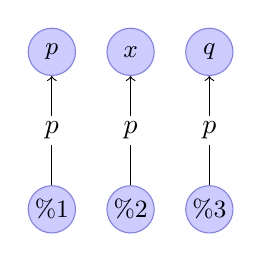
\begin{tikzpicture}[baseline=0]
            \tikzstyle{node}=[circle, draw=blue!50, fill=blue!20, inner sep=1pt, minimum size=6mm]
            \tikzstyle{linenode}=[pos=0.5,fill=white,inner sep=2pt,outer sep=2pt]
            \node[node] (A) at (0,-2) {\small$\%1$};
            \node[node] (B) at (1,-2) {\small$\%2$};
            \node[node] (C) at (2,-2) {\small$\%3$};
            \node[node] (Ap) at (0,0) {\small$p$};
            \node[node] (Bp) at (1,0) {\small$x$};
            \node[node] (Cp) at (2,0) {\small$q$};
            \path [->] (A) edge[] node[linenode] {$p$} (Ap);
            \path [->] (B) edge[] node[linenode] {$p$} (Bp);
            \path [->] (C) edge[] node[linenode] {$p$} (Cp);
        \end{tikzpicture}                                                        \\
        \midrule
        \begin{minipage}[t]{0.5\textwidth}
            \begin{minted}{llvm}
store i32* %2, i32** %1, align 8
            \end{minted}
        \end{minipage} & 
        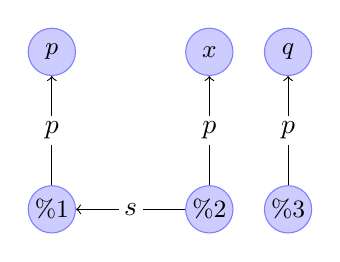
\begin{tikzpicture}[baseline=0]
            \tikzstyle{node}=[circle, draw=blue!50, fill=blue!20, inner sep=1pt, minimum size=6mm]
            \tikzstyle{linenode}=[pos=0.5,fill=white,inner sep=2pt,outer sep=2pt]
            \node[node] (A) at (0,-2) {\small$\%1$};
            \node[node] (B) at (2,-2) {\small$\%2$};
            \node[node] (C) at (3,-2) {\small$\%3$};
            \node[node] (Ap) at (0,0) {\small$p$};
            \node[node] (Bp) at (2,0) {\small$x$};
            \node[node] (Cp) at (3,0) {\small$q$};
            \path [->] (A) edge[] node[linenode] {$p$} (Ap);
            \path [->] (B) edge[] node[linenode] {$p$} (Bp);
            \path [->] (C) edge[] node[linenode] {$p$} (Cp);
            \path [->] (B) edge[] node[linenode] {$s$} (A);
        \end{tikzpicture}                                                        \\
        \midrule
        \begin{minipage}[t]{0.5\textwidth}
            \begin{minted}{llvm}
%4 = load i32*, i32** %1, align 8
store i32* %4, i32** %3, align 8
; create constraints from every 
; instruction
            \end{minted}
        \end{minipage}  & 
        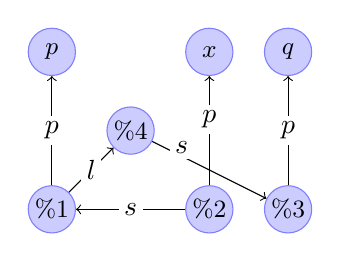
\begin{tikzpicture}[baseline=0]
            \tikzstyle{node}=[circle, draw=blue!50, fill=blue!20, inner sep=1pt, minimum size=6mm]
            \tikzstyle{linenode}=[pos=0.5,fill=white,inner sep=2pt,outer sep=2pt]
            \node[node] (A) at (0,-2) {\small$\%1$};
            \node[node] (B) at (2,-2) {\small$\%2$};
            \node[node] (C) at (3,-2) {\small$\%3$};
            \node[node] (Ap) at (0,0) {\small$p$};
            \node[node] (Bp) at (2,0) {\small$x$};
            \node[node] (Cp) at (3,0) {\small$q$};
            \node[node] (D) at (1,-1) {\small$\%4$};
            \path [->] (A) edge[] node[linenode] {$p$} (Ap);
            \path [->] (B) edge[] node[linenode, yshift=4pt] {$p$} (Bp);
            \path [->] (C) edge[] node[linenode] {$p$} (Cp);
            \path [->] (B) edge[] node[linenode] {$s$} (A);
            \path [->] (A) edge[] node[linenode] {$l$} (D);
            \path [->] (D) edge[] node[linenode, xshift=-10pt, yshift=8pt] {$s$} (C);
            % \draw[->, rounded corners=6mm] (E) -- ($(E.30) + (0.5,0.5)$) -- ($(Cp.30) + (0.4,0.4)$) node[linenode]{$s$} -- ($(C.30) + (0.5,0.5)$) -- (C);
        \end{tikzpicture} \\
        \midrule
        \begin{minipage}[t]{0.5\textwidth}
            \begin{minted}{llvm}
; apply first store 
; constraint rule(s)
            \end{minted}
        \end{minipage}               & 
        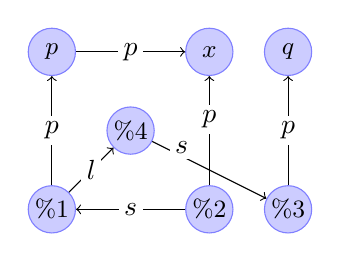
\begin{tikzpicture}[baseline=0]
            \tikzstyle{node}=[circle, draw=blue!50, fill=blue!20, inner sep=1pt, minimum size=6mm]
            \tikzstyle{linenode}=[pos=0.5,fill=white,inner sep=2pt,outer sep=2pt]
            \node[node] (A) at (0,-2) {\small$\%1$};
            \node[node] (B) at (2,-2) {\small$\%2$};
            \node[node] (C) at (3,-2) {\small$\%3$};
            \node[node] (Ap) at (0,0) {\small$p$};
            \node[node] (Bp) at (2,0) {\small$x$};
            \node[node] (Cp) at (3,0) {\small$q$};
            \node[node] (D) at (1,-1) {\small$\%4$};
            \path [->] (A) edge[] node[linenode] {$p$} (Ap);
            \path [->] (B) edge[] node[linenode, yshift=4pt] {$p$} (Bp);
            \path [->] (C) edge[] node[linenode] {$p$} (Cp);
            \path [->] (B) edge[] node[linenode] {$s$} (A);
            \path [->] (A) edge[] node[linenode] {$l$} (D);
            \path [->] (D) edge[] node[linenode, xshift=-10pt, yshift=8pt] {$s$} (C);
            % \draw[->, rounded corners=6mm] (E) -- ($(E.30) + (0.5,0.5)$) -- ($(Cp.30) + (0.4,0.4)$) node[linenode]{$s$} -- ($(C.30) + (0.5,0.5)$) -- (C);
            \path [->] (Ap) edge[] node[linenode] {$p$} (Bp);
        \end{tikzpicture} \\
        \midrule
        \begin{minipage}[t]{0.5\textwidth}
            \begin{minted}{llvm}
; apply last load and store 
; constraint rule(s)
; 
; finally p pts-to x
; and q also pts-to x
            \end{minted}
        \end{minipage}               & 
        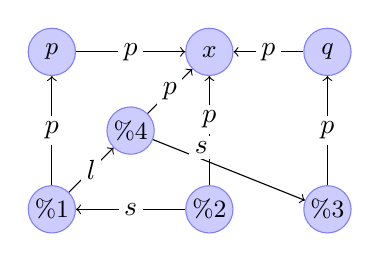
\begin{tikzpicture}[baseline=0]
            \tikzstyle{node}=[circle, draw=blue!50, fill=blue!20, inner sep=1pt, minimum size=6mm]
            \tikzstyle{linenode}=[pos=0.5,fill=white,inner sep=2pt,outer sep=2pt]
            \node[node] (A) at (0,-2) {\small$\%1$};
            \node[node] (B) at (2,-2) {\small$\%2$};
            \node[node] (C) at (3.5,-2) {\small$\%3$};
            \node[node] (Ap) at (0,0) {\small$p$};
            \node[node] (Bp) at (2,0) {\small$x$};
            \node[node] (Cp) at (3.5,0) {\small$q$};
            \node[node] (D) at (1,-1) {\small$\%4$};
            \path [->] (A) edge[] node[linenode] {$p$} (Ap);
            \path [->] (B) edge[] node[linenode, yshift=4pt] {$p$} (Bp);
            \path [->] (C) edge[] node[linenode] {$p$} (Cp);
            \path [->] (B) edge[] node[linenode] {$s$} (A);
            \path [->] (A) edge[] node[linenode] {$l$} (D);
            \path [->] (D) edge[] node[linenode, xshift=-10pt, yshift=8pt] {$s$} (C);
            % \draw[->, rounded corners=6mm] (E) -- ($(E.30) + (0.5,0.5)$) -- ($(Cp.30) + (0.4,0.4)$) node[linenode]{$s$} -- ($(C.30) + (0.5,0.5)$) -- (C);
            \path [->] (Ap) edge[] node[linenode] {$p$} (Bp);
            \path [->] (D) edge[] node[linenode] {$p$} (Bp);
            \path [->] (Cp) edge[] node[linenode] {$p$} (Bp);
        \end{tikzpicture} \\
        \bottomrule
    \end{tabular}
\end{table}

go through instrs, and how they are relevant to pta, explain constraints \cite{lin2015alias}
\section{Related Work}
\subsection{Context Free Languages}
first general idea: \cite{reps1998program} first idea of gemm for cflpq \cite{azimov2018context} kronecker product idea \cite{orachev2020context} evaluation \cite{mishin2019evaluation} spbla library \cite{orachev2021spbla}, current draft [Taming Transitive Redundancy for Context-Free Language Reachability] fron SVF, parallel pta via cfl \cite{su2014parallel}
\subsection{Sequential Analyses}
\subsubsection{SVF}
svf idea, built on top of llvm, \cite{sui2016svf}, briefly explain all subcomponents i.e. memleak detection: \cite{sui2014detecting} demand driven VF: \cite{sui2018value} new alternative, faster, better results than svf \cite{shi2018pinpoint}
\subsection{GPU Accelerated Analyses}
\subsubsection{Graspan}
original idea \cite{zheng2008demand} big data approach on cpu \cite{wang2017graspan} and gpu \cite{zuo2021systemizing} alternative impl \cite{gu2020towards} based on \cite{mendez2012gpu} and \cite{mendez2010parallel}
\section{Motivation}
general alias analysis is undecidable
This thesis aims to explore the possibilities of parallelizing the Andersen style inclusion based whole program pointer analysis. The goal is to improve static pointer analysis performance by using massively parallel GPUs.
With the general trend of more complex software systems in software development, developers also require static analysis tools that are able to perform scalable analyses on entire codebases.
Unfortunately general pointer analysis is undecidable problem, which is a problem that prevents maximally precise pointer analysis from being a possibility.
For this reason a balance must be found between performance and precision when analyzing code.
Historically most pointer analysis solutions have been implemented as single threaded applications. By using GPGPUs the proposed library from this thesis aims to improve performance when analyzing entire programs by distributing the work accross the many streaming processors modern GPGPUs possess. The proposed performance improvement also does not decrease the analysis precision.
\subsection{Static Analysis in Software Development}
finding bugs is becoming harder

inter procedural analysis scalability; create a single machine implementation that used parallel hardware and integrates into SVF

\begin{figure}
    \centering
    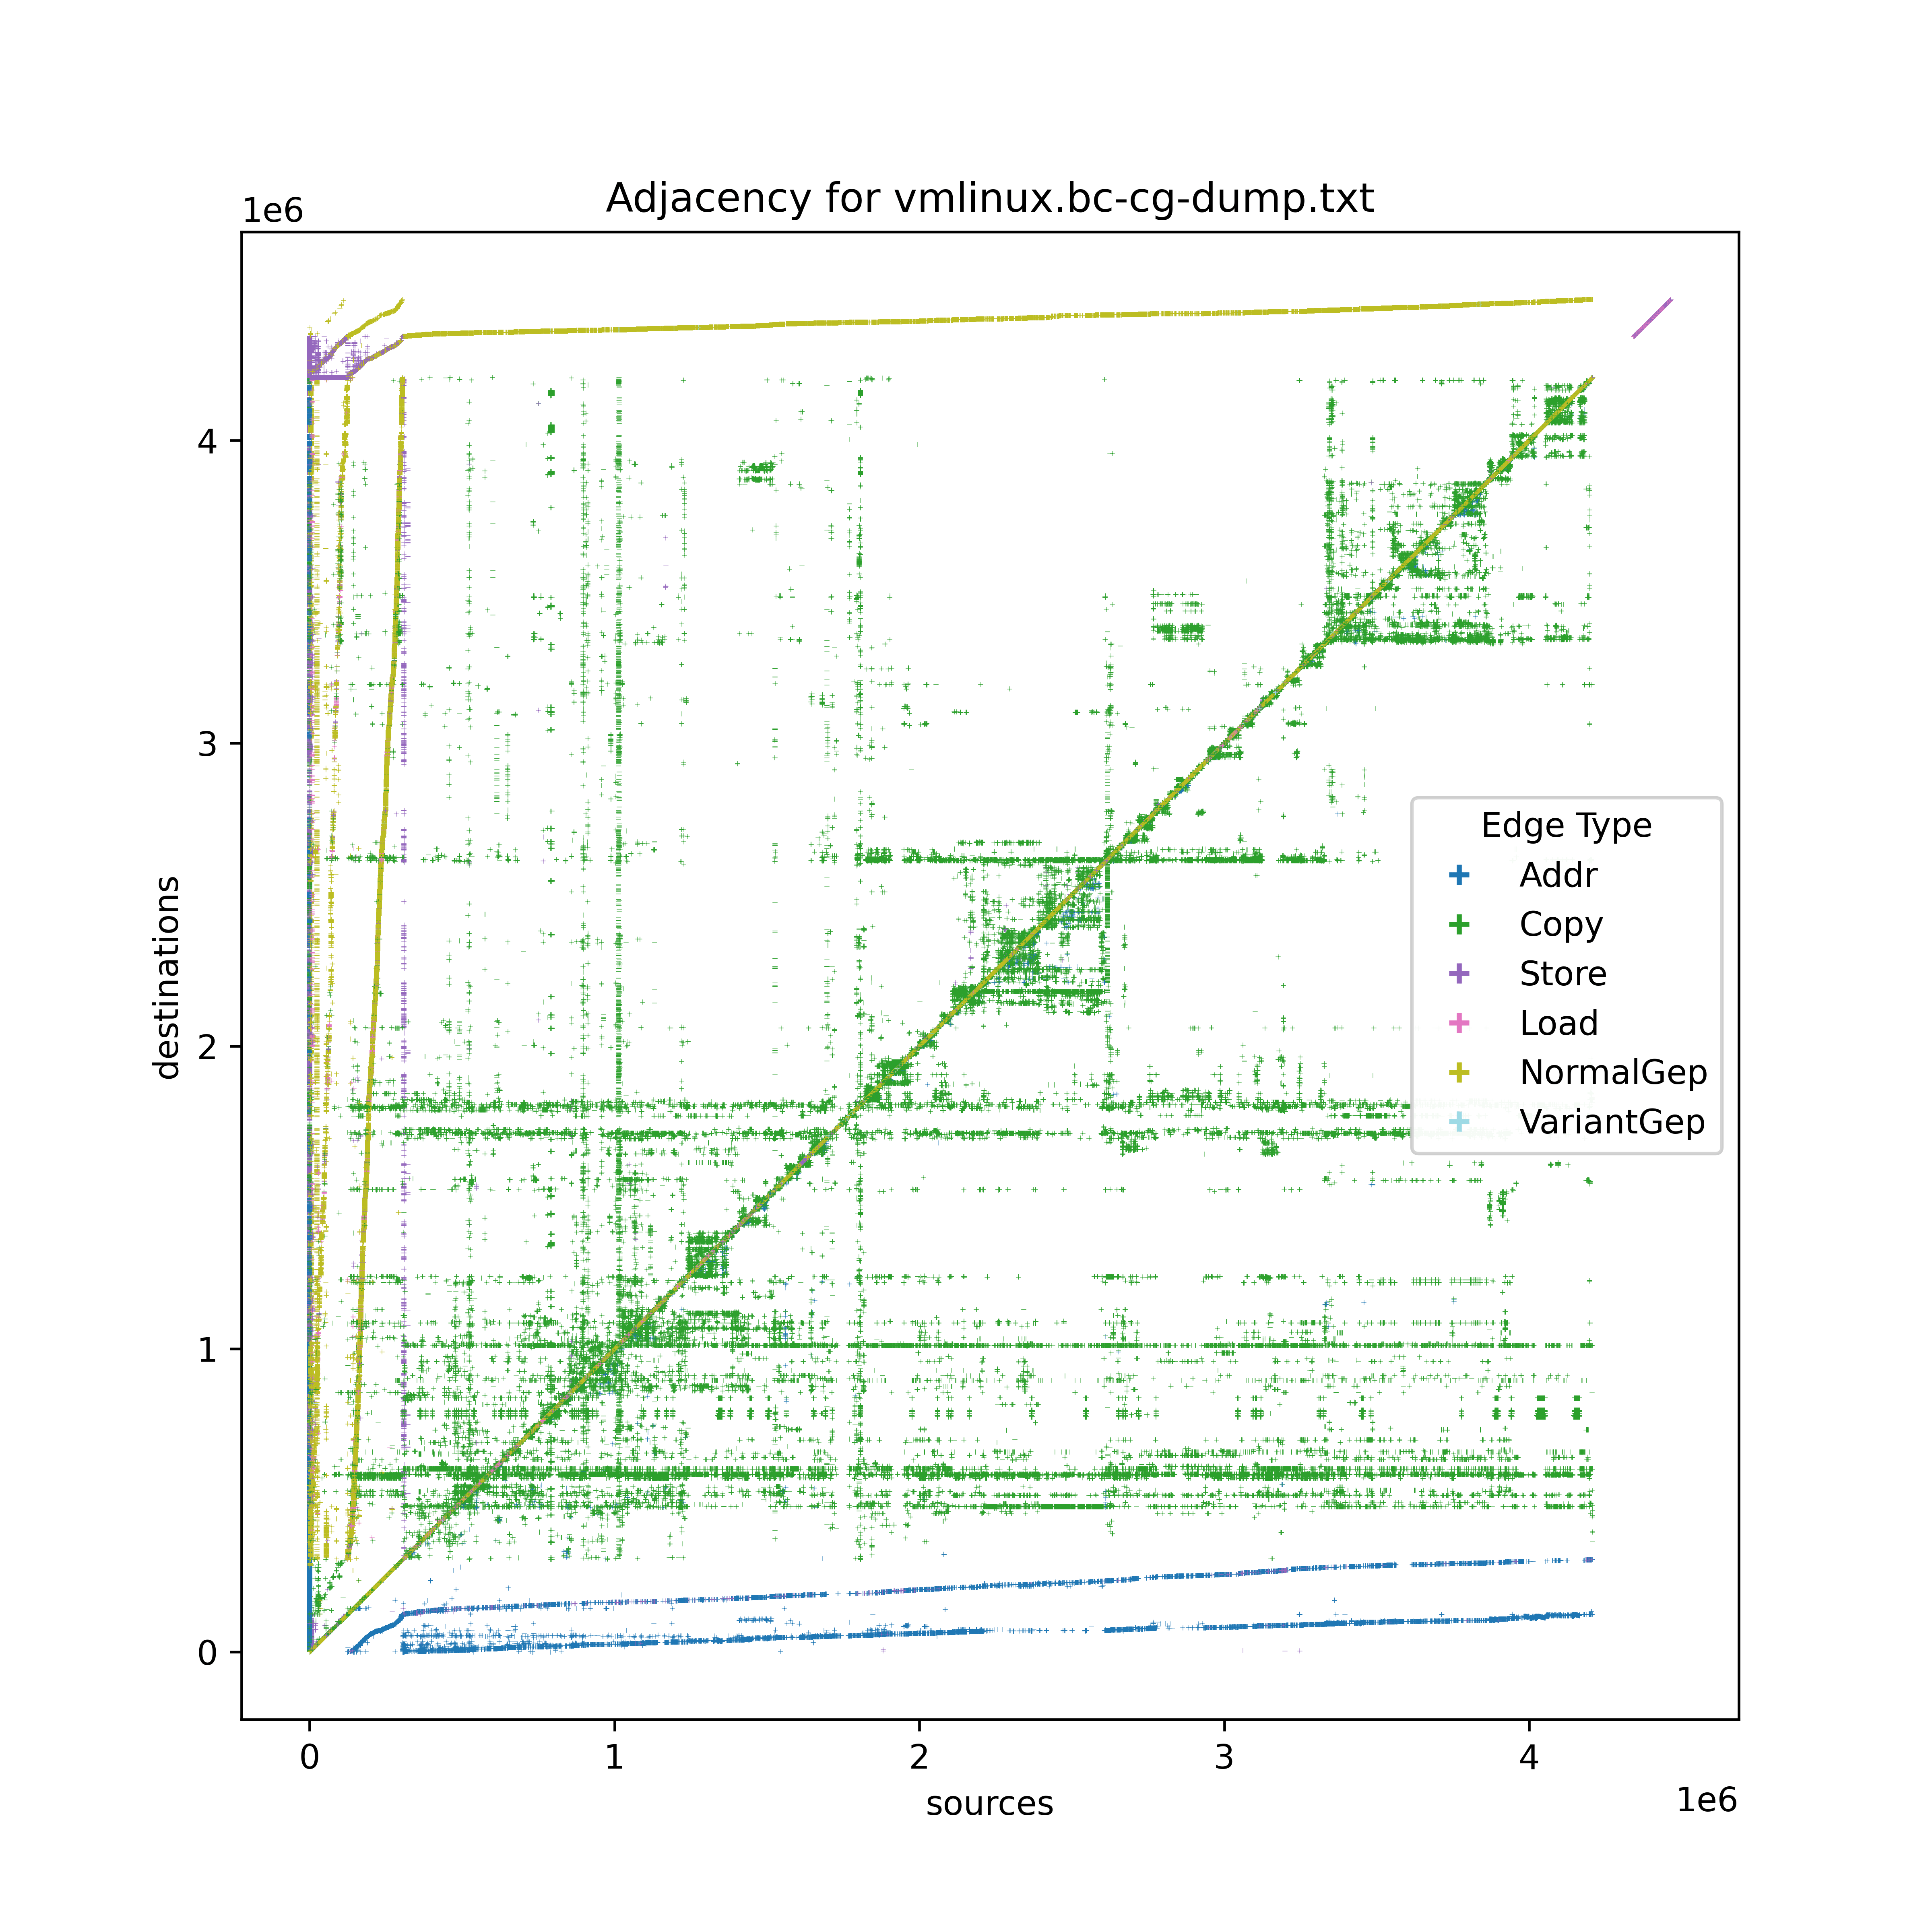
\includegraphics[width=1.\textwidth]{img/linux-consg-min.png}
    \caption{Adjacency Plot for the Constraint Graph of the Linux Kernel}
    \label{fig:linux-consg}
\end{figure}


\begin{table}
    \begin{center}
        \caption{More rows.}
        \label{tab:table1}
        \begin{tabular}{l|S|r}
            \textbf{Value 1} & \textbf{Value 2} & \textbf{Value 3} \\
            $\alpha$         & $\beta$          & $\gamma$         \\
            \hline
            1                & 1110.1           & a                \\
            2                & 10.1             & b                \\
            3                & 23.113231        & c                \\
            4                & 25.113231        & d                \\ % <-- added row here
        \end{tabular}
    \end{center}
\end{table}
